\documentclass[conference]{IEEEtran}
\IEEEoverridecommandlockouts
% The preceding line is only needed to identify funding in the first footnote. If that is unneeded, please comment it out.
\usepackage{cite}
\usepackage{amsmath,amssymb,amsfonts}
\usepackage{algorithmic}
\usepackage{graphicx}
\usepackage{textcomp}
\usepackage{url}
\usepackage{xcolor}
\usepackage{booktabs}
\usepackage{float}
\usepackage{tikz}
\usetikzlibrary{arrows.meta,calc,positioning}
\def\BibTeX{{\rm B\kern-.05em{\sc i\kern-.025em b}\kern-.08em
    T\kern-.1667em\lower.7ex\hbox{E}\kern-.125emX}}

\begin{document}

\title{Knowledge Distillation and Quantization-Aware Training for Fundus Image Classification on Embedded FPGAs}

\author{\IEEEauthorblockN{Leonardo Tisato}
\IEEEauthorblockA{\textit{Dipartimento di Elettronica, Informazione e Bioingegneria} \\
\textit{Politecnico di Milano}\\
Milano, Italy \\
leonardo.tisato@mail.polimi.it}
}

\maketitle

\begin{abstract}
Deploying neural classifiers for fundus images on embedded FPGAs requires
compressing both the network and its arithmetic while preserving the diagnostic
performance that makes the classifier useful. This work studies that tradeoff for
a four-class ultra-widefield fundus task, where the target device is an
Ultra96-v2 and the classifier must distinguish healthy eyes, choroidal nevus,
uveal melanoma, and congenital hypertrophy of the retinal pigment epithelium. We
start from a large ResNet-50 teacher and compress it into a much smaller student by
means of teacher-assistant knowledge distillation, then train low-precision
versions of the student with quantization-aware training in Brevitas and compile
the resulting networks with FINN. The hardware exploration shows that the binding
constraint is on-chip memory rather than arithmetic logic: bit-width, FIFO memory
style, and late-stage channel width determine whether the design fits and how
much layer-level parallelism can be afforded. The exploration produces two
deployable 6-bit accelerator families and several hardware operating points.
Preserving the student's original channel widths gives the highest deployed
accuracy, 81.20\%, but saturates block RAM and reaches 6.36 images/s at the
routed 187.5\,MHz clock. Reducing the late channel widths lowers accuracy only
slightly, to 80.45\%, while freeing enough memory for an additional folding step.
The best reduced-width operating point reaches 79.89 weighted F1, 75.62 macro F1,
and 12.71 images/s at 187.5\,MHz on the 133-image test set.
\end{abstract}

\begin{IEEEkeywords}
knowledge distillation, quantization-aware training, FPGA, FINN, Brevitas, embedded inference, fundus image classification
\end{IEEEkeywords}

\section{Introduction}
\label{sec:introduction}

Early differentiation of uveal melanocytic lesions is clinically decisive: uveal
melanoma is malignant and time-sensitive, yet on fundus imaging it is hard to
separate from benign nevus or congenital hypertrophy of the retinal pigment
epithelium (CHRPE), and expert reading is subject to high inter-observer
variability \cite{chadwick2025ai}. Deep learning provides reproducible decision support, and recent
work attains strong four-class accuracy on ultra-widefield fundus images
\cite{tasso2026lesion}. These systems, however, are built on large convolutional
backbones and assume workstation- or cloud-class compute, which sits awkwardly
with the point-of-care setting in which screening is most valuable.

Bringing such a classifier onto an embedded FPGA would place inference at the
bedside, at low power and latency and without transferring sensitive images
off-device. The obstacle is one of scale. Accurate models in this domain rely on
ResNet-class networks whose weight and activation memory exceeds the on-chip
budget of a small device, where block RAM is the binding resource. Compression and low-bit quantization are therefore
mandatory, yet accuracy cannot be traded away freely: a missed melanoma carries a
direct clinical cost, so a deployment is useful only if it preserves diagnostic
quality. The problem is thus to locate the operating point, in model size and
arithmetic precision, that fits the device while keeping accuracy clinically
acceptable, a balance that the strong class imbalance of the data makes harder
still.

We address this tradeoff with three contributions:
\begin{itemize}
\item a teacher-assistant knowledge-distillation chain of decreasing capacity that
  compresses the network, where an intermediate assistant suppresses the
  degradation incurred when a large teacher is distilled directly into a small
  student \cite{hinton2015distilling, cho2019efficacy, mirzadeh2020takd};
\item a Brevitas-based study of quantization-aware training across multiple
  weight and activation bit-widths \cite{pappalardo2023brevitas};
\item an end-to-end deployment through the FINN dataflow toolchain
  \cite{umuroglu2017finn, blott2018finnr} in a resource-driven design-space
  exploration over arithmetic precision and layer width, the axes that raise
  accuracy as they grow and free on-chip memory as they shrink.
\end{itemize}

On the Ultra96, the design-space exploration produces two deployable 6-bit
accelerator families rather than a single winner. One operating point preserves
more model capacity and favors accuracy, but remains memory-bound; the other
trades a small accuracy margin for enough on-chip memory headroom to add
parallelism and improve throughput. Both deployed accelerators remain bit-exact
with their software references; the fastest point reaches 12.71 images/s at
187.5\,MHz on the 133-image test set.

\section{Background}
\label{sec:background}

\subsection{Knowledge Distillation}
\label{sec:bg-kd}

Knowledge distillation transfers the behaviour of a trained teacher network to a
smaller student by training the student to match the teacher's softened output
distribution rather than the hard labels alone \cite{hinton2015distilling}. The
softened targets, obtained by raising the softmax temperature, carry the relative
confidence the teacher assigns across classes, a richer signal than a one-hot
label, and the student minimizes a weighted sum of the ordinary cross-entropy and
a distillation term that aligns the two distributions. A compact student can thus
reach an accuracy it would not attain from the labels alone, which is what makes
distillation attractive when the model to be trained is small.

The benefit, however, is not monotone in the teacher's strength. When the teacher
is much larger than the student, the student cannot reproduce its distribution and
accuracy degrades instead of improving, an effect attributed to the capacity gap
between the two networks \cite{cho2019efficacy}. The gap can be bridged with
intermediate models of decreasing size: a teaching assistant is distilled from
the large teacher and in turn teaches the student, so that each step spans a
smaller capacity gap \cite{mirzadeh2020takd}. This staged distillation is the
principle behind the teacher-assistant scheme described in
Section~\ref{sec:method-kd}.

\subsection{Neural Network Quantization}
\label{sec:bg-quant}

Quantization replaces the floating-point weights and activations of a network
with low-precision fixed-point values, reducing both the memory the model occupies
and the cost of its arithmetic. A quantizer maps a real value to a finite integer
grid defined by a scale, a zero point when the representation is asymmetric, and a
bit-width. The smaller the grid, the cheaper the hardware, but also the larger the
rounding and clipping error that the network must tolerate.

Two strategies are common. Post-training quantization starts from an already
trained floating-point network and fixes the quantizer parameters afterwards. In
practice, this means calibrating activation ranges on representative data and
mapping each weight tensor to the nearest values on the low-bit grid, by scaling,
rounding to integer codes, and clipping to the representable range. It is cheap
because it does not require another optimization run, but at low bit-widths the
induced error is often too large for the original weights to absorb.
Quantization-aware training instead inserts fake quantizers during training. A
model can still be warm-started from a floating-point checkpoint, but the
low-precision operations are simulated in the forward pass while full-precision
parameters are retained for the gradient update. The network therefore learns
weights that tolerate the precision it will use at inference
\cite{jacob2018quantization}. It costs more to train but loses far less accuracy,
particularly at low bit-widths, so we use it throughout, through Brevitas, a
PyTorch library that inserts quantized layers and exports the trained model to a
quantized ONNX graph \cite{pappalardo2023brevitas}.

\subsection{FPGA Dataflow Inference}
\label{sec:bg-fpga}

FINN implements a quantized network as a streaming dataflow accelerator. Each
layer becomes its own hardware block, and the blocks form a pipeline through which
activations flow, so that every layer is busy on a different piece of data at the
same time \cite{umuroglu2017finn}. This organization suits low-precision networks,
because their arithmetic reduces to small fixed-point operations that map directly
onto the fabric's lookup tables and DSP slices, and the fewer the bits, the less
logic each operation costs. The original FINN targeted binarized networks; its
successor FINN-R generalizes the flow to arbitrary low bit-widths, and is the
toolchain we use \cite{blott2018finnr}.

The generated graph contains both compute blocks and stream-management blocks.
The compute blocks perform the layer arithmetic, mainly through matrix-vector
activation units for convolutional and fully connected layers and thresholding
blocks for quantized activations. The stream-management blocks prepare and move
data between them: padding and input-generation blocks arrange feature maps for
convolutions, data-width converters adapt how many bits are carried per cycle,
and FIFOs buffer values between neighbouring blocks with different rates. The
important point is that the non-arithmetic blocks are not free. In a fully
on-chip accelerator, weights, thresholds, and inter-layer buffers all compete for
FPGA memory, so stream management can become as relevant as the arithmetic itself.

The accelerator exposes a few parameters that trade throughput against resource
use. For matrix-vector activation units, folding is controlled by the PE and SIMD
factors. PE replicates output-channel processing, while SIMD replicates
input-channel processing inside each dot product. Raising either factor reduces
the number of cycles needed by the corresponding layer, but consumes more lookup
tables, registers, DSP slices, and often more on-chip memory for weights or
buffers. Between consecutive blocks, FIFO buffers absorb the mismatch in their
production and consumption rates and keep the pipeline from stalling. Because the
accelerator keeps all weights and these FIFOs on chip, the limited on-chip block
RAM bounds what fits, together with the logic; which of the two binds first
depends on the network and the folding chosen.

\section{Methodology}
\label{sec:methodology}

\subsection{Dataset and Preprocessing}
\label{sec:method-data}

We use the same four-class dataset as Tasso et al.~\cite{tasso2026lesion}: 864
ultra-widefield fundus images labelled healthy, choroidal nevus, uveal melanoma,
or CHRPE, with 302, 290, 170, and 102 images per class. Uveal melanoma and CHRPE
are the least represented, and CHRPE, the smallest class, is also the hardest to
classify, as it overlaps visually with nevus. The test set holds 133 images, with
47 healthy, 44 nevus, 26 melanoma, and 16 CHRPE.

Their pipeline resizes each image to $512\times512$ and normalizes it with
ImageNet statistics, and the teacher and assistant networks
(Section~\ref{sec:method-kd}) keep this unchanged. The deployed student instead
runs at $160\times160$, the native resolution of its backbone, reached by trimming
the dark border around the circular field of view and resizing; the normalization
is the same.

\begin{figure*}[t]
\centering
\resizebox{0.95\textwidth}{!}{%
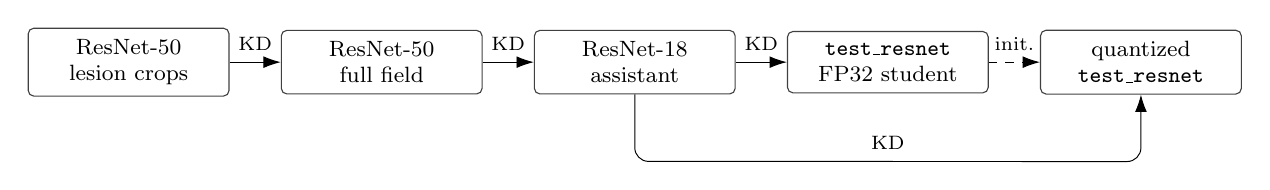
\begin{tikzpicture}[
    font=\footnotesize,
    stage/.style={
        draw=black!75,
        rounded corners=2pt,
        align=center,
        minimum width=2.55cm,
        minimum height=0.78cm,
        inner xsep=5pt,
        inner ysep=4pt
    },
    flow/.style={-{Latex[length=2.2mm,width=1.5mm]}, line width=0.35pt},
    qattrain/.style={flow, rounded corners=5pt},
    init/.style={flow, dashed},
    edge note/.style={font=\scriptsize, inner sep=0pt}
]
\node[stage] (crop) {ResNet-50\\lesion crops};
\node[stage, right=0.65cm of crop] (field) {ResNet-50\\full field};
\node[stage, right=0.65cm of field] (assistant) {ResNet-18\\assistant};
\node[stage, right=0.65cm of assistant] (student) {\texttt{test\_resnet}\\FP32 student};
\node[stage, right=0.65cm of student] (quantized) {quantized\\\texttt{test\_resnet}};

\draw[flow] (crop) -- node[midway, above=4pt, edge note] {KD} (field);
\draw[flow] (field) -- node[midway, above=4pt, edge note] {KD} (assistant);
\draw[flow] (assistant) -- node[midway, above=4pt, edge note] {KD} (student);
\draw[init] (student) -- node[midway, above=4pt, edge note] {init.} (quantized);
\draw[qattrain] (assistant.south) -- ++(0,-0.85)
    -- node[midway, above=4pt, edge note] {KD}
    ($(quantized.south)+(0,-0.85)$) -- (quantized.south);
\end{tikzpicture}%
}
\caption{The teacher-assistant distillation chain.}
\label{fig:takd}
\end{figure*}

\subsection{Teacher-Assistant Knowledge Distillation}
\label{sec:method-kd}

The deployed network must be small enough to fit the FPGA, which constrains the
architecture before accuracy is considered. On a dataset this small, training from
scratch forces a bad trade: a large network overfits, and a small one learns too
little. ImageNet-pretrained initialization avoids it by giving a small network
visual features it could not acquire from the data alone. For the deployable
student we need this initialization in a backbone much smaller than the ResNet
teachers. We therefore instantiate the student with timm using the pretrained
\texttt{test\_resnet.r160\_in1k} checkpoint hosted on Hugging Face
\cite{hfTestResnet}: a ResNet-style model with native $160\times160$ resolution
and ImageNet-1k weights. Fine-tuning it on the four-class task
improves on the small from-scratch baselines but plateaus short of the accuracy
we require, which is what motivates distillation.

Following Tasso et al., we first train a ResNet-50 \cite{he2016resnet} on
lesion-centered crops and use it to teach a ResNet-50 operating on the full
fundus field. This full-field ResNet-50 is the large teacher used for the
remaining chain. Distilling it directly into \texttt{test\_resnet} did not reach
the accuracy we expected, which is unsurprising when teacher and student are this
far apart in capacity: the student cannot match the much larger teacher's output
distribution \cite{cho2019efficacy}. The established remedy is to bridge the gap
with an intermediate network \cite{mirzadeh2020takd}, so we distil the full-field
ResNet-50 into a ResNet-18 and make that the teacher of \texttt{test\_resnet}.
Figure~\ref{fig:takd} shows the resulting teacher-assistant chain.

Every stage minimizes the same objective, a convex combination of the
cross-entropy on the labels and a Kullback-Leibler term that aligns the student's
softened output with the teacher's,
\begin{equation}
\mathcal{L} = \alpha\,\mathcal{L}_{\mathrm{CE}}(y, p_s)
            + (1-\alpha)\,\mathcal{L}_{\mathrm{KL}}(p_t^{\tau}, p_s^{\tau}),
\end{equation}
with $p_t^{\tau}$ and $p_s^{\tau}$ the teacher and student outputs softened at
temperature $\tau$, and $\alpha$ the weight on the two terms. We keep
$\alpha = 0.25$ and $\tau = 3$ throughout, including the quantization-aware
training of Section~\ref{sec:method-qat}, where distillation stays active.

\subsection{Quantization-Aware Training}
\label{sec:method-qat}

For deployment the fine-tuned student is reimplemented in Brevitas
\cite{pappalardo2023brevitas}, its convolutions, activations, and final linear
layer replaced by quantized counterparts that constrain weights and activations to
a fixed bit-width. We initialize this quantized model from the FP32 student and
run a calibration pass to set the quantizer scales. Loading the weights transfers
the trained floating-point solution into the Brevitas model; calibration then
defines how activations, and the already-loaded weights, are mapped to the
available fixed-point grid. We then continue training with quantizers active. The
distillation objective and the same teacher remain in use, so the network adapts
its weights to the precision it will use at inference instead of relying only on
the calibrated quantized warm start.

We train one model per precision, quantizing weights and activations to the same
width at 8, 6, and 4 bits. Lower precision yields a smaller accelerator but
degrades accuracy, a trade-off we examine in Section~\ref{sec:res-qat}.

\subsection{Hardware Compilation and Deployment}
\label{sec:method-hw}

The trained quantized model is exported from Brevitas to QONNX and handed to FINN,
which compiles it into the streaming dataflow accelerator described in
Section~\ref{sec:bg-fpga}: every layer becomes its own hardware block, lowered
through high-level synthesis into a bitstream. The target is the Ultra96, a Zynq
UltraScale+ device, where the programmable logic holds the accelerator and the
processing system streams images to it and reads back predictions.

FINN exposes many build parameters; those that drive the memory and throughput
trade-off we faced are the folding of the compute blocks and their adjacent stream
adapters, controlled mainly through PE and SIMD factors; the depth of each
inter-layer FIFO; the memory style of each block, that is whether its storage
maps to block RAM or to distributed LUT memory, configurable per block and
otherwise left to a default heuristic; and the target clock period. We tune these
in the design-space exploration of Section~\ref{sec:res-dse};
Section~\ref{sec:res-hw} reports the deployed configurations.

Block RAM is worth a closer look, since it turns out to be the resource that bounds
our design. The FPGA fabric used here exposes it as 36-Kb primitives, each usable
as two independent 18-Kb halves and accessed through one write and one read port.
The hardware blocks generated by FINN need storage for weights, thresholds, and
inter-layer streams. Through memory-style attributes, FINN can steer that storage
toward block RAM or distributed LUT memory, depending on the block and backend. In
the design space exploration we exploit this configurability
specifically on FIFOs, where it is a direct way to relieve BRAM pressure without
changing arithmetic. This matters
especially for shallow FIFOs, which can reserve a block-RAM primitive or half
primitive while storing only a small fraction of its capacity. FINN leaves the
FIFO memory style to a default heuristic that sends FIFOs below a depth threshold
to LUT memory and the rest to block RAM, and that assignment is the lever we act
on in Section~\ref{sec:res-dse}.

\section{Experimental Results}
\label{sec:results}

\subsection{Experimental Setup}
\label{sec:res-setup}

All designs target the Ultra96-v2, a Zynq UltraScale+ ZU3EG device. Its
programmable logic provides 70{,}560 LUTs, 141{,}120 flip-flops, 360 DSP slices,
and 216 block-RAM tiles of 36\,Kb, with no UltraRAM; these bounds are the budget
against which we report utilization.

We evaluate on the 133-image test set. On imbalanced data, overall accuracy is an
incomplete summary: it is dominated by the larger classes and says nothing about
how errors distribute across them. We therefore report macro-averaged precision,
recall, and F1, and take macro F1 as the primary metric, since it averages the
classes with equal weight so that the minority classes count as much as the
majority. For the deployed models we also report weighted F1, to summarize the
test-set performance under the observed class frequencies, and add the per-class
precision, recall, and F1, which show how the errors distribute across the
classes. Macro values are bootstrap means over the test set, while accuracy and
weighted F1 are point values. 

\subsection{Knowledge Distillation}
\label{sec:res-kd}

Table~\ref{tab:kd} lists the full-precision macro-averaged metrics along the kept distillation
chain: the lesion-crop ResNet-50, the full-field ResNet-50 it teaches, the
ResNet-18 assistant, and the final student. The deployable \texttt{test\_resnet}
is small enough that distilling the full-field teacher into it directly triggers
the capacity-gap degradation of Section~\ref{sec:method-kd}. The intermediate
ResNet-18 assistant mitigates it: in a controlled comparison, distilling the
student through the assistant rather than straight from the teacher raises its
macro F1 by about nine points, the recovery the capacity-gap argument predicts
when teacher and student differ too much in size. Distilled through the assistant,
the student reaches 79.70 accuracy and 73.92 macro F1 at the $160\times160$
input.

\begin{table}[H]
\centering
\caption{The distillation chain.}
\label{tab:kd}
\begin{tabular}{lcccc}
\toprule
Model & Acc & Prec. & Rec. & F1 \\
\midrule
ResNet-50 (lesion-crops)   & 88.72 & 87.45 & 87.83 & 87.38 \\
ResNet-50 (full field)    & 92.48 & 94.22 & 89.68 & 91.39 \\
ResNet-18 (assistant)           & 90.98 & 91.20 & 88.41 & 89.30 \\
\texttt{test\_resnet} & 79.70 & 85.00 & 71.69 & 73.92 \\
\bottomrule
\end{tabular}
\end{table}

\subsection{Quantization and Bit-Width Exploration}
\label{sec:res-qat}

Table~\ref{tab:qat} lists the macro-averaged metrics of \texttt{test\_resnet} at
full precision and after QAT, with weights and activations quantized to the same
width. Both 8-bit and 6-bit QAT preserve the full-precision accuracy: each reaches
81.20 accuracy, above the 79.70 full-precision baseline. The 6-bit run is slightly
stronger on the macro metrics, reaching 76.39 macro F1 against 75.97 for 8 bits,
so reducing precision from 8 to 6 bits does not introduce an accuracy penalty in
software. At 4 bits training fails to recover, the validation macro F1 stalling
around 60.

\begin{table}[H]
\centering
\caption{Full-width quantization.}
\label{tab:qat}
\begin{tabular}{lcccc}
\toprule
Precision & Acc & Prec. & Rec. & F1 \\
\midrule
Full precision & 79.70 & 85.00 & 71.69 & 73.92 \\
8-bit          & 81.20 & 81.71 & 74.19 & 75.97 \\
6-bit          & 81.20 & 82.74 & 74.34 & 76.39 \\
\bottomrule
\end{tabular}
\end{table}

\subsection{Design Space Exploration}
\label{sec:res-dse}

For our network the binding resource is block RAM: logic and DSP slices stay
comfortably within budget, but on-chip memory does not, so fitting the accelerator
is a problem of block-RAM allocation. Following the mechanism described in
Section~\ref{sec:method-hw}, we map FIFOs below a depth threshold to LUTRAM and
leave deeper FIFOs in block RAM, where they use the primitives more efficiently.
This memory-style relief is the step that brings the design within the device:
without it the accelerator overruns the available block RAM at every precision,
and with it block-RAM utilization is the measure that separates the configurations
that fit from those that do not.

\begin{figure}[H]
\centering
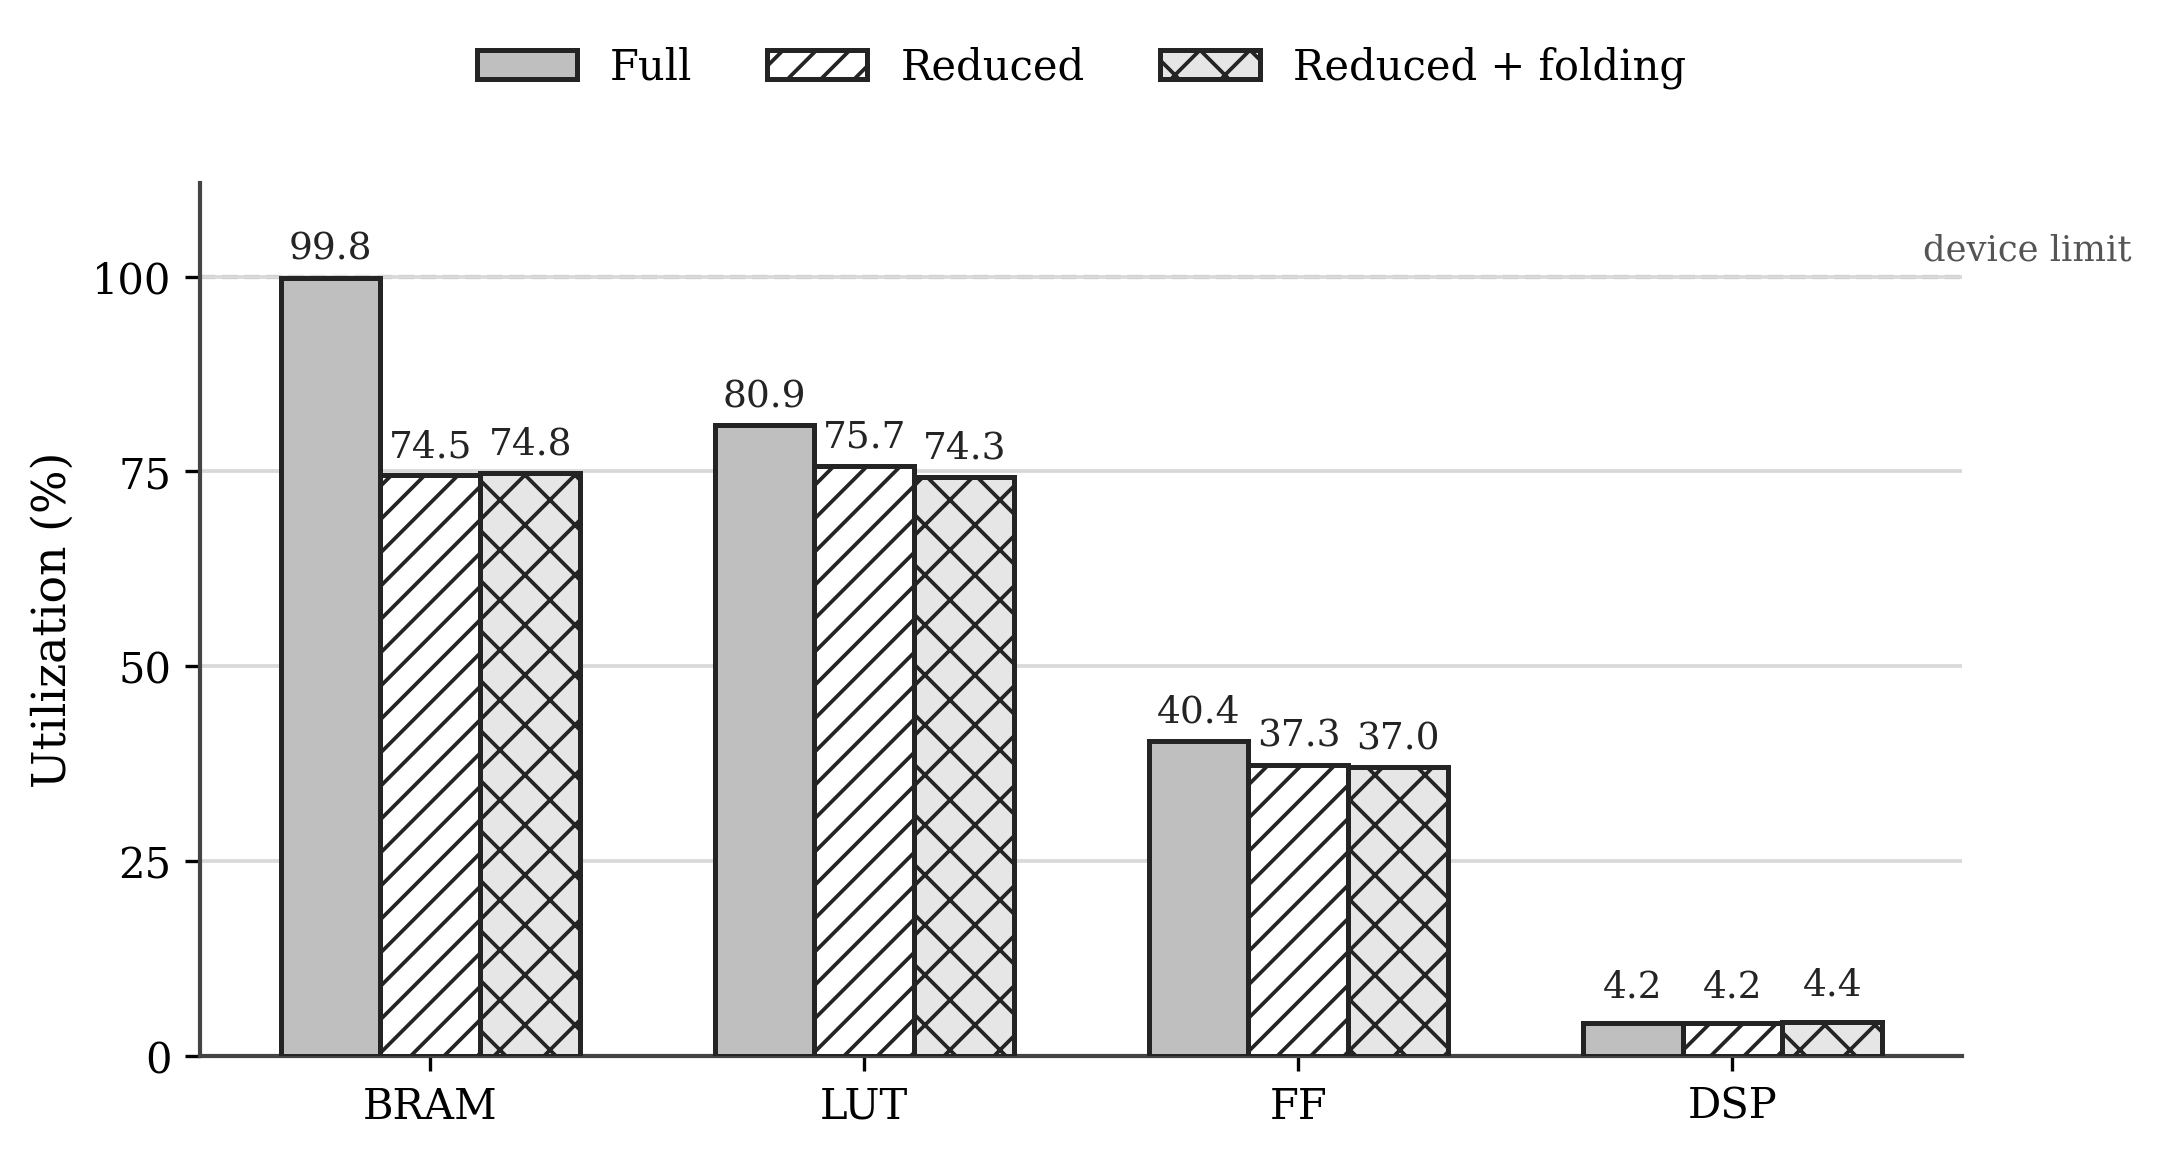
\includegraphics[width=\columnwidth]{figures/resource_utilization.png}
\caption{Resource projection.}
\label{fig:resource-util}
\end{figure}

With the relief applied throughout, the three precisions behave differently on the
full \texttt{test\_resnet}. At 8 bits the wider weights and activations overutilize
both block RAM and LUTRAM under the FINN configurations we evaluated, so that
precision is not deployable. At 6 bits the accelerator fits, with block RAM at
99.8\%, LUTs at 80.9\%, and flip-flops and DSPs far from full
(Figure~\ref{fig:resource-util}). At 4 bits accuracy has already collapsed
(Section~\ref{sec:res-qat}), so that precision is never built. Six bits is thus the
only setting that both fits the device and preserves accuracy, and is therefore
our first deployable design. This design uses the baseline FINN folding point for
the matrix-vector units, with PE and SIMD set to 1. Since block RAM
is already at 99.8\%, there is no practical headroom for increasing those factors.

\begin{table}[H]
\centering
\caption{Reduced-width quantization.}
\label{tab:slim}
\begin{tabular}{lcccc}
\toprule
Precision & Acc & Prec. & Rec. & F1 \\
\midrule
Full precision & 80.45 & 82.22 & 72.00 & 74.11 \\
8-bit          & 81.20 & 80.06 & 75.75 & 76.86 \\
6-bit          & 80.45 & 79.01 & 74.77 & 75.62 \\
\bottomrule
\end{tabular}
\end{table}

To trade a small accuracy margin for the headroom that more parallelism needs, we
introduce a narrowed variant, the \texttt{slim\_test\_resnet}, whose last two
channel widths are reduced from 192 and 96 to 128 and 64, then retrained under the
same distillation and QAT procedure. Table~\ref{tab:slim} reports its software
accuracy. At full precision it reaches 80.45 accuracy and 74.11 macro F1, 0.75
points of accuracy below the full network. The 8-bit QAT model reaches 81.20
accuracy and 76.86 macro F1. At 6 bits, the model holds 80.45 accuracy and 75.62
macro F1. As at full width, 4-bit training collapses and is discarded.

On hardware the reduced-width model repeats this bit-width pattern. At 8 bits it
still overutilizes block RAM and LUTRAM, as the full network does, so the most
accurate configuration again does not fit. At 6 bits it fits with room to spare: the
narrower stages reduce weight storage, bringing block RAM to about 74.5\% before
any extra folding. We do not prescribe a custom per-layer folding configuration;
instead, we raise FINN's target-FPS parameter until its automatic folding pass
selects the first additional parallelization step. This keeps block RAM at
74.8\%; more aggressive target-FPS values were also tested, but the FIFO depths
selected by FINN grew enough to overutilize block RAM again. LUTs and flip-flops slightly
decrease, while DSP use stays essentially unchanged except for the one additional
unit introduced by the folded reduced-width design
(Figure~\ref{fig:resource-util}). Six bits is therefore the precision we deploy,
now with the block-RAM headroom for useful parallelism that the full model lacked.
Figure~\ref{fig:resource-util} therefore reports three resource configurations:
the full-width graph, the reduced-width graph, and the reduced-width graph after
the selected extra folding.

\begin{table}[H]
\centering
\caption{Timing report.}
\label{tab:timing}
\footnotesize
\begin{tabular}{llrrr}
\toprule
Model & Build & Req. & Impl. & WNS \\
\midrule
Full    & unfolded & 100 & 100   & $+4.21$ \\
        & unfolded & 200 & 187.5 & $+0.30$ \\
\midrule
Reduced & unfolded & 100 & 100   & $+3.70$ \\
        & folded   & 100 & 100   & $+4.13$ \\
        & folded   & 200 & 187.5 & $+0.19$ \\
\bottomrule
\end{tabular}
\end{table}

Every build in Table~\ref{tab:timing} meets timing at its implemented clock; the
requested and implemented clocks are in MHz and WNS is in ns. The full network
closes without extra folding at 100\,MHz with 4.21\,ns of slack and at
187.5\,MHz with 0.30\,ns of slack. The reduced-width network first closes without
extra folding at 100\,MHz with 3.70\,ns of slack. After the selected folding step,
it still closes at 100\,MHz, with 4.13\,ns of slack, and reaches 187.5\,MHz with
0.19\,ns of slack when the clock target is tightened. We therefore use
187.5\,MHz as the deployed clock: it is the fastest frequency reached by the flow
with positive slack and is already close to the timing limit.

\subsection{Hardware Deployment Results}
\label{sec:res-hw}

The design-space exploration leaves two deployable 6-bit accelerator families on
the Ultra96: the full-width \texttt{test\_resnet}, which gives the highest board
accuracy, and the reduced-width variant, which sacrifices a small accuracy margin
for the memory headroom needed by folding. Clock and folding do not change the
quantized weights or the predicted labels, so classification performance is
reported once per family. In both cases the deployed hardware is bit-exact with
its software reference on the 133-image test payload.

\begin{table}[H]
\centering
\caption{Deployment accuracy.}
\label{tab:deployment}
\begin{tabular}{lrrr}
\toprule
Family & Acc & wF1 & mF1 \\
\midrule
Full    & 81.20 & 80.39 & 76.77 \\
Reduced & 80.45 & 79.89 & 75.62 \\
\bottomrule
\end{tabular}
\end{table}

Table~\ref{tab:deployment} gives the on-board accuracy view. The full-width
family reaches 81.20 accuracy and 76.77 macro F1, while the reduced-width family
reaches 80.45 accuracy and 75.62 macro F1. The cost of the reduced-width design
is therefore 0.75 percentage points of accuracy, with almost no movement in
weighted F1. The per-class breakdown in Table~\ref{tab:per-class} shows where
that residual error lies.

\begin{table}[H]
\centering
\caption{Per-class deployment metrics.}
\label{tab:per-class}
\begin{tabular}{llrrrr}
\toprule
Family & Class & n & Prec. & Rec. & F1 \\
\midrule
Full & Healthy  & 47 & 78.3  & 100.0 & 87.8 \\
     & Nevus    & 44 & 80.0  & 81.8  & 80.7 \\
     & Melanoma & 26 & 100.0 & 65.4  & 78.7 \\
     & CHRPE    & 16 & 72.6  & 50.2  & 58.4 \\
\midrule
Reduced & Healthy  & 47 & 82.5 & 100.0 & 90.3 \\
     & Nevus    & 44 & 79.1 & 77.3  & 78.0 \\
     & Melanoma & 26 & 94.5 & 65.5  & 77.0 \\
     & CHRPE    & 16 & 60.0 & 56.3  & 57.2 \\
\bottomrule
\end{tabular}
\end{table}

Neither family collapses on any class. Both recover every healthy image, and
nevus remains balanced between precision and recall. The clinically harder
minority classes carry most of the residual error. Melanoma precision stays high
in both families, but recall remains close to 65\%, so missed malignancies are
the main clinical weakness. CHRPE is the weakest class by F1 in both families,
consistent with its small support and its visual overlap with nevus.

The throughput results show the effect of the freed memory on folding. The
full-width family keeps the baseline FINN folding point and reaches
3.39 images/s at 100\,MHz and 6.36 images/s at the routed 187.5\,MHz clock. The
reduced-width family is first measured without extra folding at 100\,MHz, where
it matches the same 3.39 images/s baseline. After the automatic folding step
selected in Section~\ref{sec:res-dse}, it reaches 6.78 images/s at 100\,MHz and
12.71 images/s at 187.5\,MHz (Figure~\ref{fig:deployment-throughput}).

\begin{figure}[H]
\centering
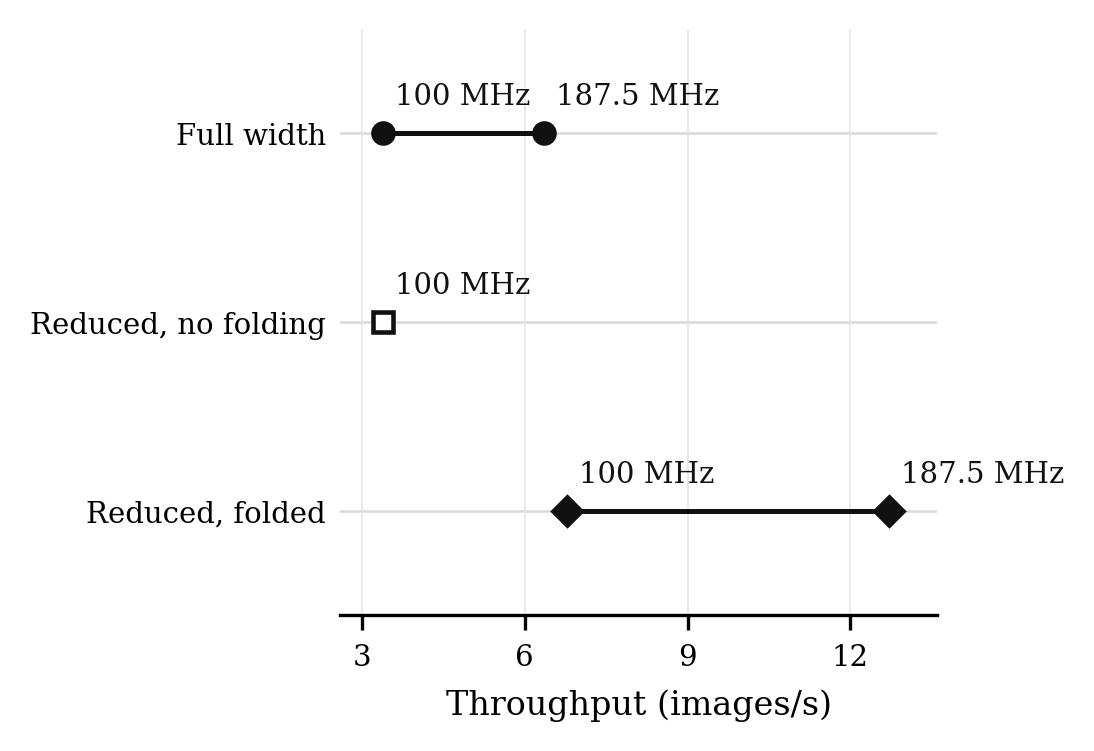
\includegraphics[width=\columnwidth]{figures/deployment_tradeoff.png}
\caption{Throughput operating points.}
\label{fig:deployment-throughput}
\end{figure}

The gain at the fastest clock is therefore not a clock-only effect: both families
are evaluated at 187.5\,MHz, but the reduced-width graph has enough memory margin
for the extra folding step. This raises throughput from 6.36 to 12.71 images/s at
the same clock, at the 0.75-point accuracy cost reported above.

\section{Conclusion}
\label{sec:conclusion}

This work combines teacher-assistant distillation, low-bit quantization-aware
training, and FINN dataflow compilation to obtain a deployable Ultra96
accelerator for the four-class ultra-widefield fundus task. The intermediate
ResNet-18 assistant was needed to avoid the capacity-gap loss observed when the
large teacher was distilled directly into the tiny student. Six-bit QAT preserved
the student's accuracy while reducing the arithmetic precision enough for FPGA
deployment.

The hardware exploration was ultimately limited by on-chip memory rather than
compute. Moving selected FIFOs from block RAM to LUTRAM made the full 6-bit
\texttt{test\_resnet} fit, but it left almost no block-RAM headroom for extra
folding. The reduced-width variant narrowed the late channel widths, freed memory,
and enabled one additional folding point. The resulting operating points span
clock scaling and folding: at the same 187.5\,MHz clock, throughput rose from
6.36 images/s for the full model to 12.71 images/s for the reduced-width model,
with board accuracy decreasing only from 81.20 to 80.45. The final
reduced-width accelerator is bit-exact with its software reference and reaches
79.89 weighted F1 and 75.62 macro F1.

The remaining limitations are the ones exposed by the design space itself.
Four-bit quantization collapses accuracy for this small network, 8-bit hardware
does not fit the Ultra96 resource budget, and the final deployment remains
memory-bound. The main clinical weakness is still recall on the minority lesion
classes, especially melanoma and CHRPE. Future work should therefore improve
FIFO sizing and folding selection in the FINN flow, explore architectures with
better minority-class recall at the same memory cost, and evaluate larger FPGA
devices able to host higher-resolution variants.


\bibliographystyle{IEEEtran}
\bibliography{references}

\end{document}
